\documentclass[uplatex]{jsarticle}

%% Packages
\usepackage[dvipdfmx]{graphicx,color,hyperref}
\usepackage{algorithm}
\usepackage{algorithmic}
\usepackage{url}
\usepackage{lscape}
\usepackage{mathtools}
\usepackage{here}
\usepackage{amsmath,amssymb,amsfonts}
\usepackage{amsthm}
\usepackage{pxjahyper}

%% Theorem Styles
\newtheorem{theorem}{定理}
\newtheorem{proposition}{命題}
\newtheorem{cor}{系}
\newtheorem{definition}{定義}
\newtheorem{problem}{問題}
\theoremstyle{remark}
\newtheorem{remark}{注意}
\newtheorem{requirement}{条件}

%% Title
\title{An Empirical Evaluation of Columnar Storage Formats}
\author{\empty}
\date{\empty}

%% Document body
\begin{document}
\maketitle

\begin{itemize}
    \item Link: \url{https://dl.acm.org/doi/10.14778/3626292.3626298}
    \item Conference: VLDB2024
    \item Citation: \cite{columnar_storage_formats}
    \item Arxiv: \url{https://arxiv.org/abs/2304.05028}
\end{itemize}

\section{概要}
\begin{itemize}
  \item 2010年代ごろに提案されたカラム思考ストレージフォーマットが現代のハードウェアにとって本当によいフォーマットなのか?という点を調査した論文
  \item Parquet、ORCが良く用いられるオープンソースのカラム型ストレージフォーマットであるが、この有効性はHadoopベースのe2eな性能測定にとどまり、ある設計のトレードオフについての議論などは行われていない。
  \item この論文ではカラム型ファイルフォーマットを分析して、次世代のカラム指向ストレージフォーマット設計のために重要な点がなにかを明らかにすることを目的としている。
  \item 結論としては
  \begin{itemize}
    \item 辞書エンコーディングが実世界のデータを扱う上では重要
    \item ストレージが高速かつ低コストであるため、圧縮率よりでコード速度を重視すべき
    \item Parquet, ORCは高速化のためのデータ構造の設計が単純すぎる
    \item 現在のフォーマットは、ベクトル検索、多数の特徴量を用いた場合などの機械学習用途に対して最適化されていない。
  \end{itemize}
\end{itemize}

\section{背景}
\begin{itemize}
  \item これまでのカラム型ストレージフォーマットの性能測定の多くはファイルフォーマットの内部設計を評価するのではなく、クエリエンジン全体の処理性能を分析していた。よって、どのような設計が性能に寄与しているかといった分析は少なかった。
\end{itemize}

\section{さまざまなカラム型ストレージの特徴}
Parque, ORCが持つ特徴(設計)を体系的に分類し、共通点、相違点を説明する。

\begin{itemize}
  \item レイアウト
  \begin{itemize}
    \item 行単位でいくつかに分割して、その中でカラムごとに保存するという点は共通。この分割したものを「カラムチャンク」と呼ぶ。
    \item Parquetは「行数ベース」での分割、ORCは「バイト数ベース」での分割という違いがある。
  \end{itemize}
  \item エンコーディング
  \begin{itemize}
    \item 辞書エンコーディング、ランレングス圧縮、ビットパッキングは共通
    \begin{itemize}
      \item 辞書エンコーディングはカラムの重複しない値をすべて取り出した辞書を作り、その辞書のidを保存することで、ストレージサイズを小さくする。
      \item 辞書エンコーディングすると、カラムは小さな整数列になる。この整数のビット数を減らすことをビットパッキングという。
    \end{itemize}
    \item Parquetはデフォルトで全ての列に辞書エンコーディングを行う、辞書エンコーディングにはランレングス圧縮、ビットパッキングを行う。
    \item ORCは文字列の場合のみ辞書エンコーディングを行う。NDV比(異なる値の総数/創行数)が小さい場合のみ辞書エンコーディングを行う。
  \end{itemize}
  \item ブロック圧縮
  \begin{itemize}
    \item ブロック圧縮はエンコーディング後のデータをさらに圧縮することを指す。
    \item ORCはSnappy, zlib, LZO, zstd, LZ4をサポートしており、ParquetはSnappy, gzip, LZO, zstd, LZ4, Brotliをサポートしている。
  \end{itemize}
  \item インデックスとフィルター
  \begin{itemize}
    \item Parquet, ORCともに以下の二つに対応
    \begin{itemize}
      \item Zone map: 特定行範囲の最小値と最大値を保存することで、クエリのフィルタリングを高速化する。
      \item Bloom filter: 特定行範囲に特定の値が存在するかどうかを高速に判定するためのデータ構造。
    \end{itemize}
    \item Parquet: 最小zone map単位は物理サイズ単位, Bloom filterはカラムチャンク単位。
    \item ORC: 最小zone map単位は行数単位, Bloom filterはzone map単位。
  \end{itemize}
\end{itemize}

\begin{figure}
  \centering
  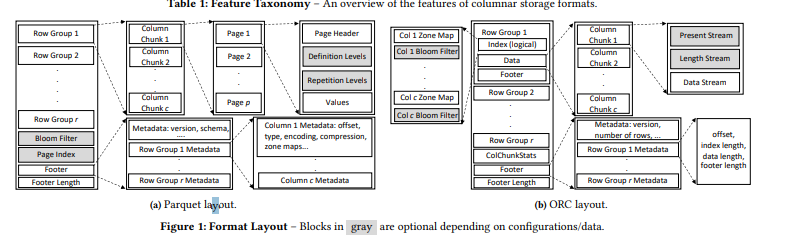
\includegraphics[width=0.5\textwidth]{img/columnar_storage_format_format.png}
  \caption{フォーマットの説明}
  \label{fig:storage-format}
\end{figure}

\section{実験}

\subsection{ベンチマークに用いたデータセット}
\begin{itemize}
  \item これまでのデータセットは実世界のデータ分布を反映しているとは言えなかったため、実世界のデータ分布を反映したベンチマークフレームワークを設計した。
  \item まずデータセットの指標を定義し、それを満たすようなデータセットを生成できるようにする。
  \item データセットの指標は以下の通り
  \begin{itemize}
    \item NDV比: 各カラムの異なる値の総数/総行数
    \item Null Ratio: 各カラムのNull値の総数/総行数
    \item Value Range: 各カラムの値の範囲
    \item Sortednes: 各カラムの値がソートされているかどうか(図\ref{fig:sortedness}参照)
    \item Skew pattern: 一様、Zipf、HotSpot、Binaryの4種類で分布の偏りを表現する。
  \end{itemize}
  \item これらの指標が現実世界のデータセットでどうなっているか調べ、それに基づいてデータを生成した。
  \item 利用したデータセットはPublic BI Benchmark, ClickHouse, UCI-ML, Yelp, LOC, Geonames, IMDbの7種類で指標は以下のようになっていた。
  \begin{itemize}
    \item NDV比: 整数、文字列カラムの80\%以上が0.01未満
    \item Null Ratio: 全体的に低め
    \item Value Range: 整数は小さい値がおおく、Bitpacking向き
    \item Sortednes: 完全にソートもしくは、完全にランダムに二極化
    \item Skew pattern: ほとんどがZipfに該当し、一様なものはほとんどない。
  \end{itemize}
  \item これをもとにデータセットを作成し、core, bi, classic, geo, log, mlの6種類のデータセットを作成した。それぞれの指標は表\ref{fig:dataset-workload}のようになっている。
\end{itemize}

\begin{figure}
  \centering
  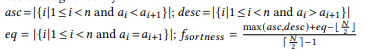
\includegraphics[width=0.5\textwidth]{img/sortedness.png}
  \caption{ソートされているかどうかの指標}
  \label{fig:sortedness}
\end{figure}

\begin{figure}
  \centering
  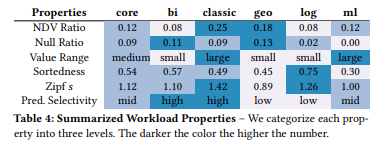
\includegraphics[width=0.5\textwidth]{img/dataset-workload.png}
  \caption{作成したデータセットの性質}
  \label{fig:dataset-workload}
\end{figure}

\subsection{ベンチマーク結果}

\begin{figure}
  \centering
  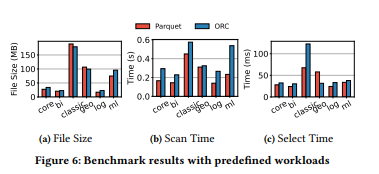
\includegraphics[width=0.5\textwidth]{img/columnar-storage-format-result1.png}
  \caption{作成したデータセットの性質}
  \label{fig:result1}
\end{figure}

\begin{itemize}
  \item 概要
  \begin{itemize}
    \item ファイルサイズ; Parquetはlog, mlで小さく、ORCはclassic, geoで小さい
    \item フルスキャン時間; Parquetの方が全体的に高速
    \item フィルタリング時間; geoではORCの方が高速、それ以外ではParquetの方が高速
  \end{itemize}
  \item エンコーディングの分析
  \begin{itemize}
    \item 圧縮率; 整数カラムの場合、NDV比が低-中程度だとParquetが有利、NDV比が高いとORCの圧縮の方がつよい(Delta, PFOR)
    \item デコード速度; 基本Parquetの方が高速、ORCはエンコーディングの切り替えがおおく、分岐予測ミスがおおい。
  \end{itemize}
  \item ブロック圧縮
  \begin{itemize}
    \item NVMeのような高速ストレージではデコードコストがI/O削減効果を上回ることがわかったため、現代の高速なストレージにおいては必ずしも圧縮は有理ではない。
  \end{itemize}
  \item フィルタ付きスキャン
  \begin{itemize}
    \item ORCのほうがzone mapの粒度が細かいので、クエリ結果のデータが少ないケースで有利。
    \item Bloom filterはORCの方が細かい粒度で構築される。
  \end{itemize}
\end{itemize}

\section{感想}
\begin{itemize}
  \item そもそもカラム型ストレージの仕組みについて知らなかったので勉強になった。行ごとに分けてからカラムごとに保存することで圧縮や高速なフィルタリングを実現しているのは面白い。
  \item データの分布やハードウェアの進歩により最適なフォーマットが違うというのはなるほどと思った。時代とともに適切なデータフォーマットも変わっていくのだなと思った。
  \item 機械学習用途として適切なデータフォーマットなど考えると面白いのではないかと思った。
\end{itemize}


\bibliographystyle{jplain}
\bibliography{template.bib}

\end{document}